%
% einleitung.tex -- Beispiel-File für die Einleitung
%
% (c) 2020 Prof Dr Andreas Müller, Hochschule Rapperswil
%
% !TEX root = ../../buch.tex
% !TEX encoding = UTF-8
%
\subsection{Kartesisch\label{geodaeten:section:Standardverfahren:Kartesisch}}
\rhead{Standardverfahren Beispiele}

Für den kartesischen Raum mit dem metrischen Tensor
 
\begin{equation}
g_{ij} = \begin{pmatrix} 
	1 & 0 \\ 
	0 & 1 
\end{pmatrix},
\end{equation}
wollen wir die Christoffel-Symbole berechnen.
Die Christoffel-Symbole sind gegeben durch

\begin{equation}
\Gamma^i_{jk} = \frac{1}{2} g^{kl} \left( \frac{\partial g_{jl}}{\partial u^i} + \frac{\partial g_{il}}{\partial u^j} - \frac{\partial g_{ij}}{\partial u^l} \right),
\end{equation}
wobei $g^{ij}$ die Inverse des metrischen Tensors ist.
Da der metrische Tensor $g_{ij}$ konstant ist und keine direkte Abhängigkeit von den Koordinaten aufweist, verschwinden alle Ableitungen.
Ohne weitere Berechnungen kann man also schliessen, dass

\begin{equation}
\frac{\partial g_{ij}}{\partial u^k} = 0 .
\end{equation}
Somit ergeben sich alle Christoffel-Symbole als null

\begin{equation}
\Gamma^i_{jk} = 0 .
\end{equation}

Denkt man an die Definition aus Abschnitt \ref{geodaeten:section:Standardverfahren}, macht dies durchaus Sinn.
Denn der Kartesische Raum ist nicht gekrümmt, weshalb keine Korrektur der Geraden notwendig ist.

Setzt man die Christoffel-Symbole in die allgemeine Geodätengleichung \eqref{geodaeten:equation:StandardverfahrenGeodaeten:Geodaetengleichung} ein, erhält man mit $u^1 = x(t)$
\begin{equation}
	\begin{alignedat}{3}
		&\ddot{u}^1 + \Gamma_{ij}^1 \dot{u}^i \dot{u}^j &\quad = \quad& 0 \\
		% &\ddot{u}^1 + 0_{ij} \cdot \dot{u}^i \dot{u}^j &\quad = \quad& 0\\
		&\ddot{u}^1  &\quad = \quad& 0 \\
		&\ddot{x}(t) &\quad = \quad& 0
	\end{alignedat}
	\label{geodaeten:equation:Standardverfahren:Kartesisch:x}
\end{equation}
und mit $u^2 = y(t)$
\begin{equation}
	\begin{alignedat}{3}
		&\ddot{u}^2 + \Gamma_{ij}^2 \dot{u}^i \dot{u}^j &\quad = \quad& 0 \\
		% &\ddot{u}^2 + 0_{ij} \cdot \dot{u}^i \dot{u}^j &\quad = \quad& 0 \\
		% &\ddot{u}^2  &\quad = \quad& 0 \\
		&\ddot{y}(t) &\quad = \quad& 0  .
	\end{alignedat}
	\label{geodaeten:equation:Standardverfahren:Kartesisch:y}
\end{equation}



Man sieht bereits, da die zweite Ableitungen in beide Dimensionen Null sind, handelt es sich bei dem kürzesten Weg um eine Gerade, was aus der Erfahrung durchaus Sinn ergibt.

Setzt man nun zwei Punkte als Start und Endpunkt, kann man durch diese Nebenbedingungen eine konkrete Lösung erhalten.
Beispielsweise wollen wir den kürzesten Weg zwischen $P_A = (1,1)$ und $P_B = (3,5)$ berechnen. 
Durch doppeltes integrieren der zweiten Ableitung von $x(t)$ erhält man

\begin{equation}
	\frac{d^2x}{dt^2} = 0 
	\Rightarrow \frac{dx}{dt} = c_1 
	\Rightarrow x(t) = c_1 \cdot t + c_2  .
	\label{geodaeten:equation:Standardverfahren:Kartesisch:equation1}
\end{equation}
Dabei sind $c_1$  und $c_2$ Integrationskonstanten. 

Wir sehen, die Gleichung entspricht einer parametrierten Geradengleichung mit $c_2$ als Startwert für $x(0)$ und $c_1$ als Steigung von $x(t)$. 
Mit $P_A(x_1,y_1)$ und $P_B(x_2,y_2)$ haben diese Gleichungen die Form

\begin{align}
	x(t) &= (x_2 - x_1) \cdot t + x_1 \\
	y(t) &= (y_2 - y_1) \cdot t + y_1
\end{align}
Da die Linie durch den Startpunkt gehen muss ist der Startwert bei $t=0$ bekannt als
 
\begin{equation}
	0 \cdot c_1 + c_2 = 1 \Rightarrow c_2 = 1 .	
\end{equation}
Die Steigung $c_1$ kann mithilfe von Endpunkt und Startpunkt berechnet werden als

\begin{equation}
	c_1 = x_2 - x_1 \\ = 3-1 \\ = 2
\end{equation}
und damit ist die Lösung der Geodätengleichung in $x$ gleich

\begin{equation}
	x(t) = 2t + 1 .
\end{equation}

Analog für $y(t)$ ist ist die Lösung der Geodätengleichung in $y$ gleich

\begin{equation}
	y(t) = 4t + 1 .
\end{equation}

\begin{figure}
	\centering
	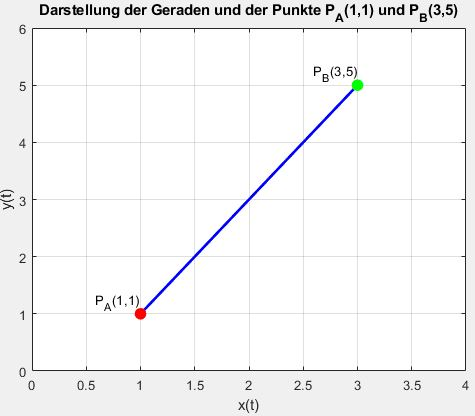
\includegraphics[width=10cm]{papers/geodaeten/Abbildungen/Standardverfahren/Kartesisch}
	\label{geodaeten:figure:Standardverfahren:Kartesisch:figure1}
	\caption{Darstellung der Kurve von x(t) und y(t) mit $t \in [0 , 1]$ Wie man sieht ist der kürzeste Weg von Punkt A zu Punkt B eine gerade.}
\end{figure}
